\section{Momentum Evaluation Model}

\subsection{Model Overview}~{}

To determine which player is performing better at a specific time, we create a indicator ``Momentum'' 
using the Analytic Hierarchy Process (AHP) to give a quantitative and overall evaluation.

Out of our own interpretation of AHP, we will break down the problems into fout parts:

\begin{enumerate}
    \item Problem Analysis
    \item Data Cleaning and Normalization
    \item Collinearity Detection
    \item Analytic Hierarchy Process (AHP)
\end{enumerate}

\subsubsection{Problem Analysis}~{}

\indent To investigate the reasons behind "momentum," we first need to provide a preliminary definition for "momentum." The magnitude of "momentum" is defined as $$f_{ijk}=\boldsymbol{\omega}\cdot\boldsymbol{x_{ijk}}$$
where:
\begin{enumerate}
    \item $f_{ijk}$ represents the "momentum" of player $k$ before the $j$th point number in the $i$th match (in the order given by the table).
    \item $\boldsymbol{x_{ijk}}$ is an $n$-dimensional column vector representing some influencing factors at the corresponding moment. Specific details will be provided later.
    \item $\boldsymbol{\omega}$ is an $n$-dimensional row vector indicating the specific weights of the influencing factors, which will be obtained through the Analytic Hierarchy Process (AHP).
    \item In this formula, there are two different calculation methods, one representing rounds where the player serves and the other representing rounds where the opponent serves. We can express it as $$\boldsymbol{\omega}=\boldsymbol{\omega_0} \circ \boldsymbol{\delta}=(\omega_0^{(0)}\delta^{(0)},\omega_0^{(1)}\delta^{(1)},\dots,\omega_0^{(n)}\delta^{(n)})$$ representing a vector formed by element-wise multiplication of two vectors of the same dimension. Here, $\boldsymbol{\delta}$ is a $0,1$ vector indicating whether it is the player's serving round. In the specific calculation, we will consider two cases separately.
\end{enumerate}

\subsubsection{Notations}~{}

\begin{table}[!h]
\centering
\begin{tabular}{cccccc}
    
    \toprule
    Symbols & Description \\ 
    \midrule
    $player$ & the current player we are considering (e.g. while calculating momentum) \\
    $point_i$ & the $i^{th}$ point of the match, a vector consists of fields stated in the given dictionary \\
    $cur$ & the current index of the point, i.e. the match is currently at the $cur^{th}$ point \\
    $H_i$ & denotes the set $\{point_{cur}, point_{cur - 1}, \ldots , point_{cur - i + 1}\}$ \\
    $S_i$ & the set of latest $i$ points where $player$ serves\\
    $R_i$ & the set of latest $i$ points where $player$ returns\\
    $P_{ace}$ & current probability of hitting an ace by $player$ \\
    $P_{df}$ & current probability of double-faulting by $player$ \\
    $P_{1st}$ & current first serve goal rate by $player$ \\
    $P_{fw}$ & current probability of $player$ winning a served point within 3 rallies \\
    $rd$ & current return depth of $player$ \\
    $P_{win}$ & current probability of hitting a winner by $player$ \\
    $P_{net}$ & current net win rate of $player$ \\
    $dist$ & $player$'s running distance on the point \\
    $P_{unf}$ & current probability of hitting an unforced error by $player$ \\
    $scored$ & whether $player$ scored the current point \\
    $diff$ & the score diffrence for $player$ in the current game (by number of points) \\
    $M$ & the current momentum of $player$ after a point \\

    \bottomrule
\end{tabular}
\end{table}
To access a certain field in a point, we simply use the field name stated in the given 
dictionary as index, i.e. for a point $point$, we use $point_{ace}$ to denote the binary 
variable that shows whether $player$ hits an ace ball in the point.


\subsubsection{Data Cleaning and Normalization}~{}

For the specific definition of $\boldsymbol{x_{ij}^{n}}$, we believe that, 
in addition to whether the player is serving, many other factors can have an impact,
including the player's skills, fatigue level, and real-time mental state of the games.
Based on these three main aspects, 
we have organized 12 factors as preliminary influencing factors, as follows:

\begin{equation}
    P_{ace} = \frac{\sum_{p \in S_3} p_{ace}}{3}
\end{equation}
\begin{equation}
    P_{df} = -\frac{\sum_{p \in S_3} p_{double\_fault}}{3}
\end{equation}
\begin{equation}
    P_{1st} = \frac{\sum_{p \in S_3} [p_{serve\_no} = 1]}{3}
\end{equation}
\begin{equation}
    P_{fw} = \frac{\sum_{p \in S_3} [p_{rally\_count} \le 3] [p_{point\_victor} = player]}{3}
\end{equation}
\begin{equation}
    rd = \frac{\sum_{p \in R_3} \left\{
        \begin{aligned}
        0, && p_{return\_depth} = ND \\
        1, && p_{return\_depth} = D \\
        -1, && p_{return\_depth} = NA \\
        \end{aligned}
        \right.}{3}
\end{equation}
\begin{equation}
    P_{win} = \frac{\sum_{p \in H_3} p_{winner}}{3}
\end{equation}
\begin{equation}
    P_{net} = \frac{\sum_{p \in H_3} p_{net\_pt\_won}}{\sum_{p \in H_3} p_{net\_pt}}
\end{equation}
\begin{equation}
    dist = \left\{
        \begin{aligned}
        0, && point_{cur, distance\_run} < 5 \\
        -1, && point_{cur, distance\_run} > 45 \\
        \frac{5 - point_{cur, distance\_run}}{40}, && otherwise \\
        \end{aligned}
        \right.
\end{equation}
\begin{equation}
    P_{unf} = -\frac{\sum_{p \in H_3} p_{unf\_err}}{3}
\end{equation}
\begin{equation}
    scored = [point_{cur, point\_victor} = player]
\end{equation}
\begin{equation}
    diff = \frac{\sum_{p \in point}[p_{set\_no} = point_{cur, set\_no}][p_{game\_no} = point_{cur, game\_no}](2[p_{point\_victor} = player]-1)}{\min\{3, \sum_{p \in point}[p_{set\_no} = point_{cur, set\_no}][p_{game\_no} = point_{cur, game\_no}]\}}
\end{equation}
\par In order to normalize the data processed, we convert the original data to limit them in $[-1, 1]$. 
For those factors that negatively influence the momentum, such as $P_{df}$, we made sure it's in $[-1, 0]$. For those factors that positively influence the momentum, such as $P_{win}$, we made sure it's in $[0, 1]$. For those factors that influence the momentum in both ways, such as $diff$, we made sure it's in $[-1, 1]$.

\subsubsection{Collinearity Detection}~{}

After processing the data, considering the potential collinearity among factors within the same category,
such as serving aces, first-serve scoring rate, and whether the previous point was scored may 
be correlated, as well as running distance and the number of strokes possibly being related, 
we conducted collinearity detection using Stata. The results of the detection indicate a
significant variance inflation factor between running distance and the number of strokes. 
Therefore, we decided to exclude one of them, choosing to retain the remaining 11 variables 
for the Analytic Hierarchy Process (AHP).

\subsubsection{Analytic Hierarchy Process}

We have previously decomposed the included factors from top to bottom into several levels, 
where factors within the same level are subordinate to factors in the level above or influence 
factors in the level above. They also dominate factors in the next level or are influenced by 
factors in the next level. Starting from the second level of the hierarchy, we construct 
comparison matrices for each factor influencing the factor in the level above, until reaching 
the bottom level. Each element in the matrix indicates the preference level between factor i and 
factor j at the same level. It is essential to note that we have separately established a series 
of such comparison matrices for two different serving types (serving by oneself and serving by 
the opponent). Here, we illustrate the matrix using serving by oneself as an example:

\begin{figure}[H]
    \centering
    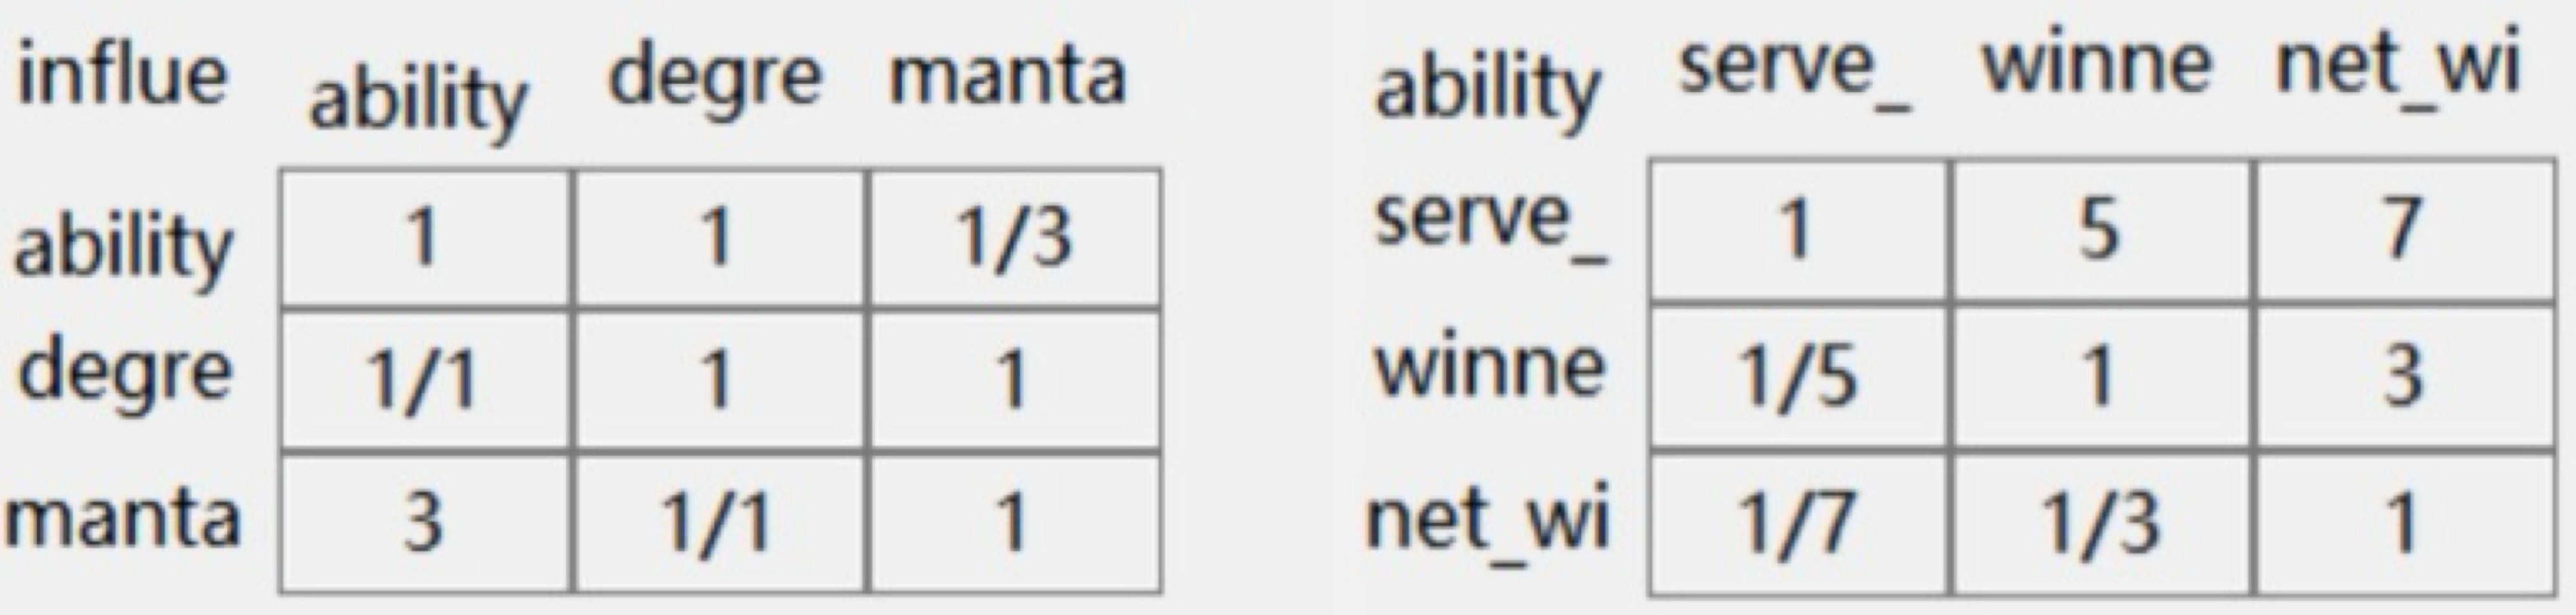
\includegraphics[scale=0.06]{mainmatter/imgs/2.jpg}
    \caption{Comparison matrix for influencing factors and ability}
\end{figure}
\begin{figure}[H]
    \centering
    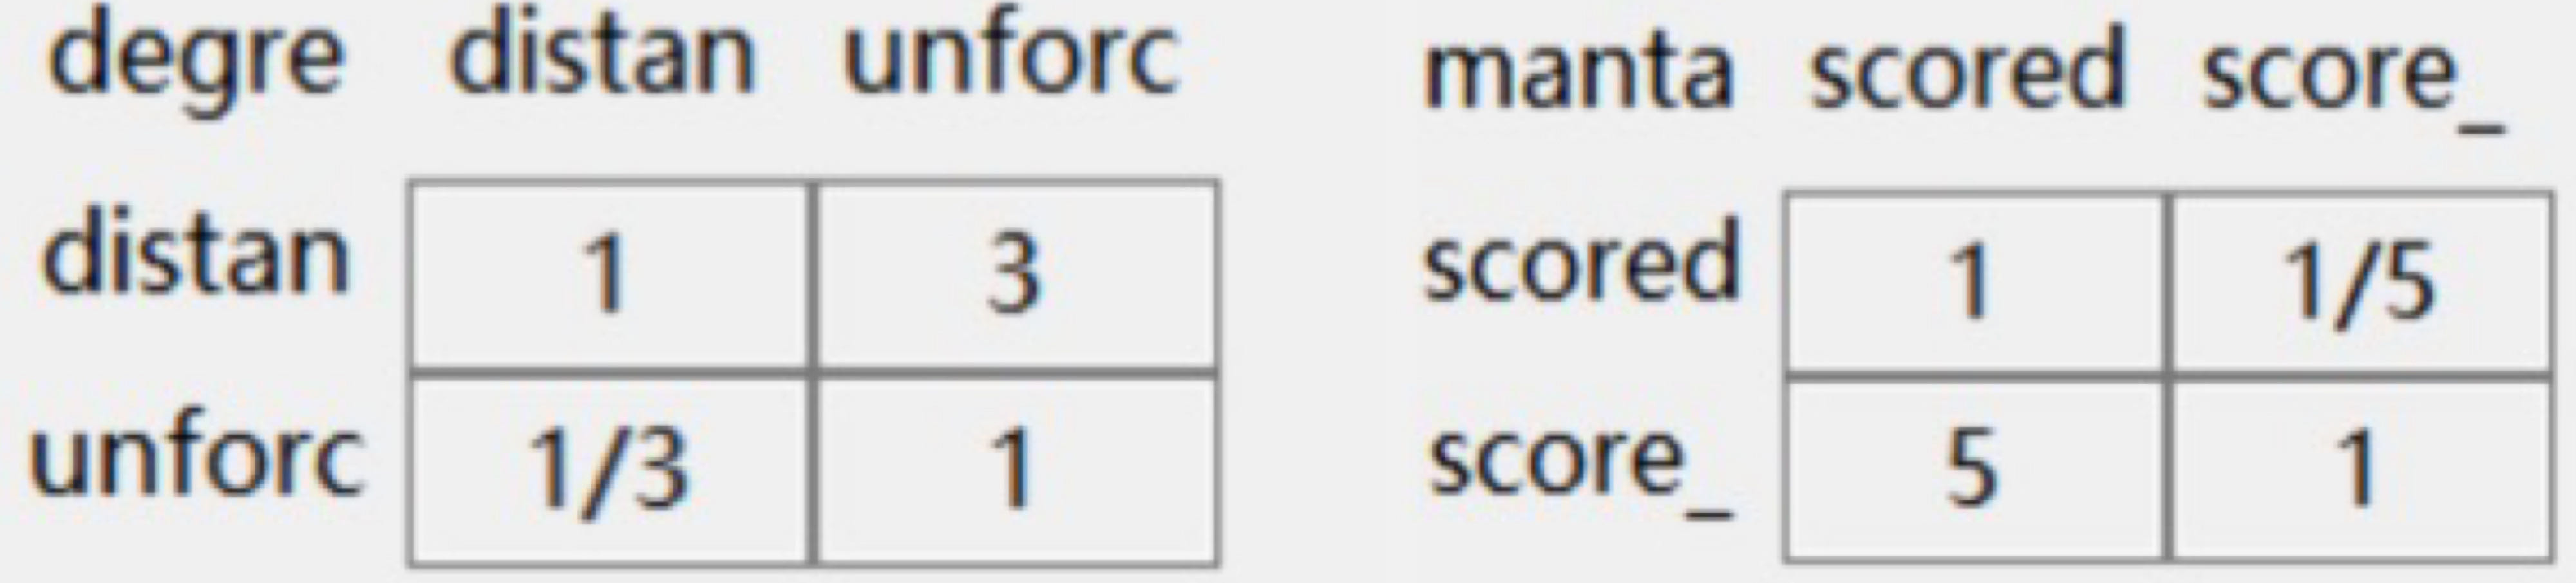
\includegraphics[scale=0.06]{mainmatter/imgs/3.jpg}
    \caption{Comparison matrix for degree of fatigue and mantality}
\end{figure}
\begin{figure}[H]
    \centering
    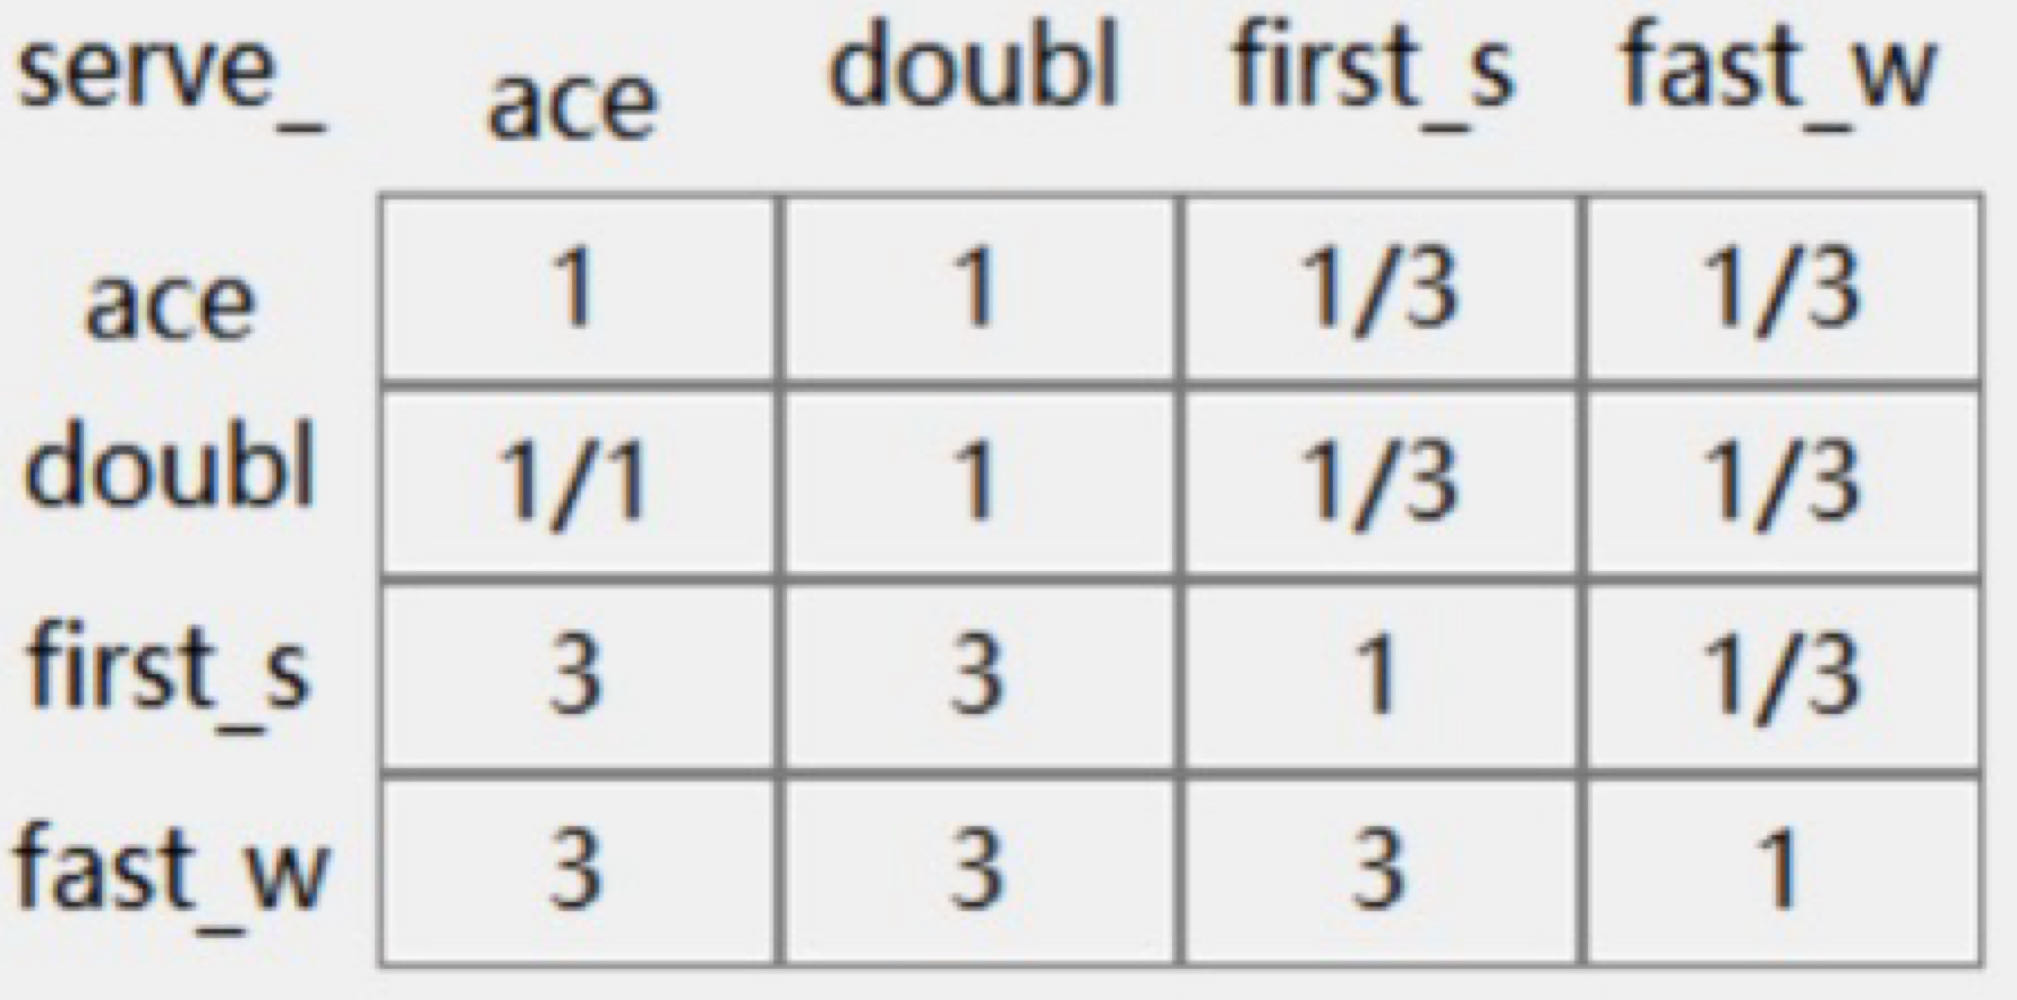
\includegraphics[scale=0.06]{mainmatter/imgs/4.jpg}
    \caption{Comparison matrix for serving}
\end{figure}

We obtain the weights for each component by calculating the maximum eigenvalue and normalizing 
its corresponding eigenvector. Certainly, for each matrix, we first need to test consistency 
using the Consistency Ratio (CR), where \(CR=\frac{CI}{RI}\), \(CI=\frac{\lambda_{max}-n}{n-1}\), 
\(RI=0.0, 0.58, 0.9\) (for matrices of size \(2, 3, 4\)). The computed Consistency Ratios for the 
matrices are 0.076, 0.037, 0.0, 0.0, 0.046. Since they are all less than 0.1, it confirms the 
consistency of the matrices.\\

\indent Therefore, the weights for our model are as follows:


\begin{figure}[H]
    \centering
    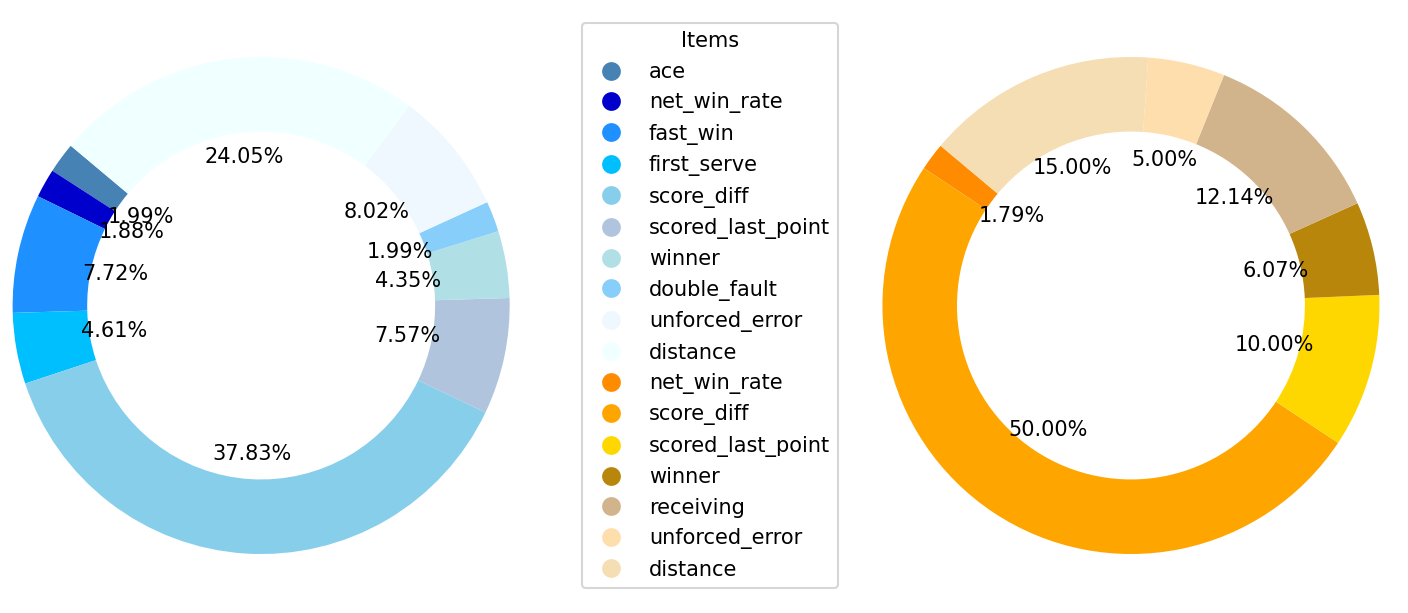
\includegraphics[scale=0.65]{mainmatter/imgs/7.png}
    \caption{Weights in two different situations}
\end{figure}

Analyzing the various factors in the chart, it is evident that the most impactful factor is 
whether the previous point was scored. Following closely is the distance covered during the 
play, which aligns well with common intuition.\\

Thus, our final momentum is defined as:(need to change symbol)
$$momentum=\begin{cases}
    \sum\limits_{n=1,n\neq 5}^{11}\omega_n x_n, & \text{if the player serves}  \\
    \sum\limits_{n=5}^{11}\omega_n x_n, & \text{if the opponent serves}
\end{cases}$$
Where $\omega_n(n=1,\dots,11)$ represent the weight of the factors, which is listed in Figure 4.\\

\subsection{Visualization and Analysis}~{}

Now, we illustrate the graph of the "momentum" in the first match:

\begin{figure}[H]
    \centering
    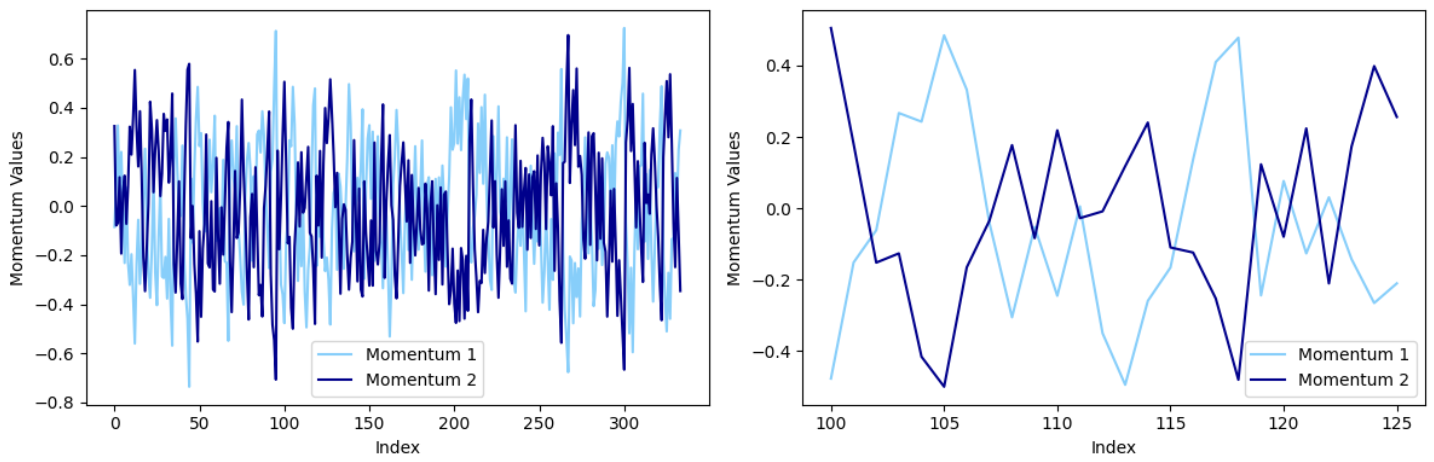
\includegraphics[scale=0.65]{mainmatter/imgs/5.png}
    \caption{Momentum change in the first competition(global and local)}
\end{figure}

It can be observed that the variation in ``momentum'' is a process of give and take.
In photo 2, when momentum 1 is above momentum 2, it means that the player 1 is performing better than the opponent. 

\subsection{momentum autocorrelation and correlation with runs of success}~{}

To answer the coach's doubt,
we need to perform autocorrelation test on momentum, 
and perform correlation test between current momentum and future scores
in this section.

If the momentum has a high autocorrelation, it means that the momentum at this moment 
has a high impact on future performance. And if the correlation between momentum and 
future scores is high, it means that the player with higher momentum has a higher
chance to win the next multiple round.

\subsubsection{momentum autocorrelation}~{}

To check if sequence of momentum is self-related, we calculate the Pearson correlation 
between momentum and that with a time lag.

\begin{algorithm}
    \caption{Calculate autocorrelation function}\label{alg:auto_corr}
    \begin{algorithmic}
        \For{$i = 1$ to $31$}
            \State $time\_series \gets momentum(i^{th}\ match\_index: {i+1}^{th}\ match\_index - 1)$
            \State $max\_lag \gets \lfloor length(time\_series) / 2 \rfloor$ \Comment{Consider lags up to half of the length of the time series}
            \State $autocorrelation \gets \text{zeros}(1, max\_lag)$

            \For{$shift = 1$ to $max\_lag$}
                \State $correlation \gets \text{corrcoef}(time\_series(1 : \text{end} - shift), time\_series(shift + 1 : \text{end}))$
                \State $autocorrelation(shift) \gets correlation(1, 2)$
            \EndFor

            \Comment{Further processing or visualization can be performed here}
        \EndFor
    \end{algorithmic}
\end{algorithm}

Here we display the autocorrelation of momentum of the first player in first three games.
There are similar results for the second player and for the momentum difference.

\begin{figure}[H]
    \centering
    \begin{subfigure}[b]{0.34\textwidth}
        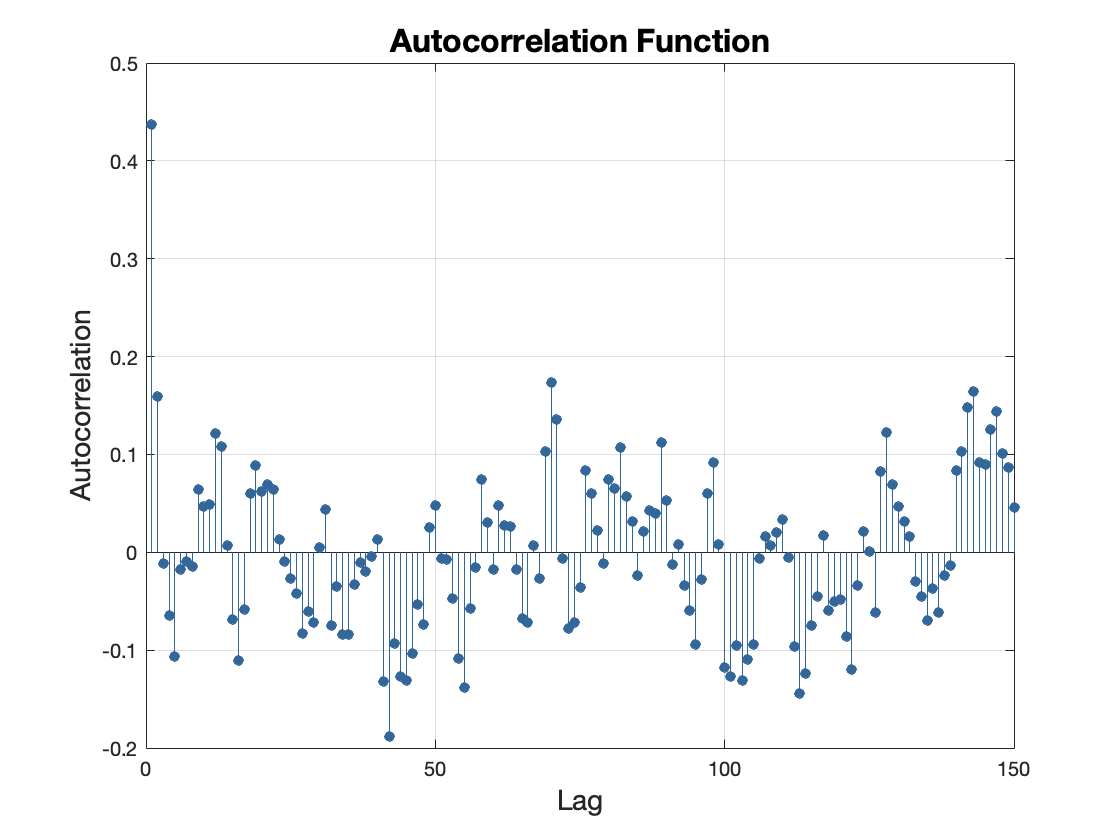
\includegraphics[width=\linewidth]{mainmatter/photos/momen_selfco_1.png}
        \caption{autocorrelation in match 1}
    \end{subfigure}\hspace{-0.02\textwidth}
    \begin{subfigure}[b]{0.34\textwidth}
        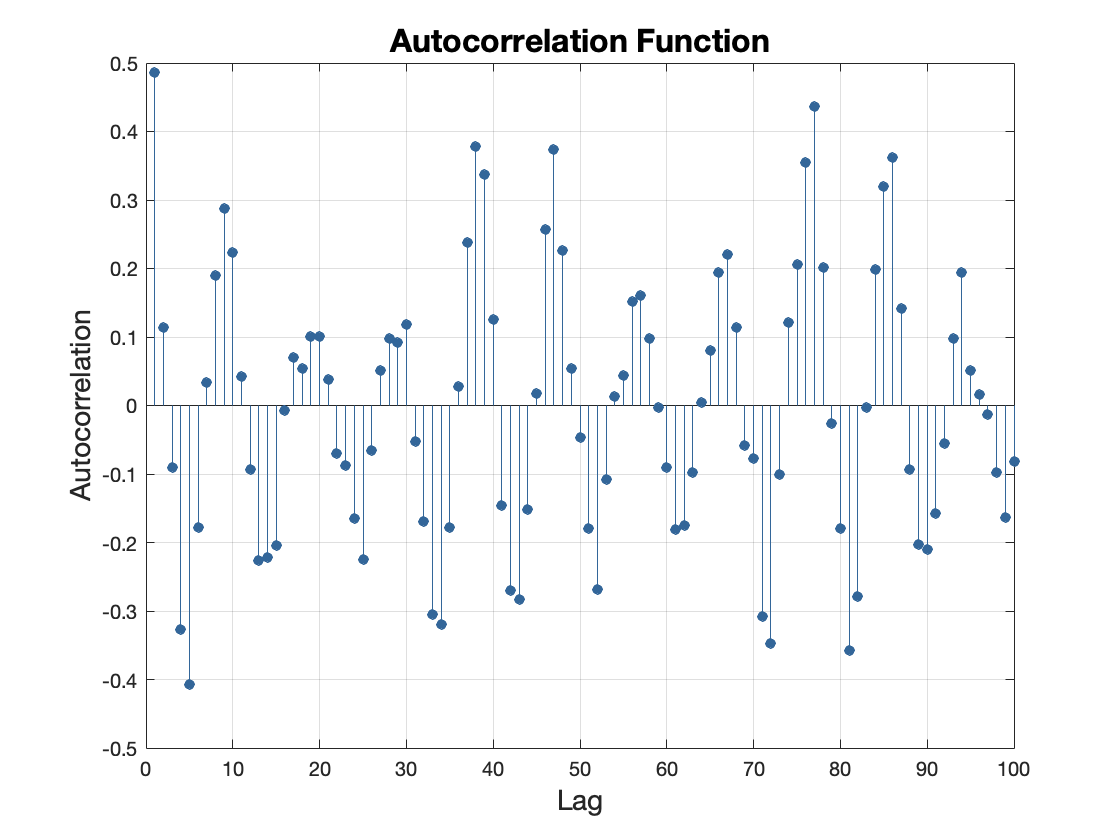
\includegraphics[width=\linewidth]{mainmatter/photos/momen_selfco_2.png}
        \caption{autocorrelation in match 2}
    \end{subfigure}\hspace{-0.02\textwidth}
    \begin{subfigure}[b]{0.34\textwidth}
        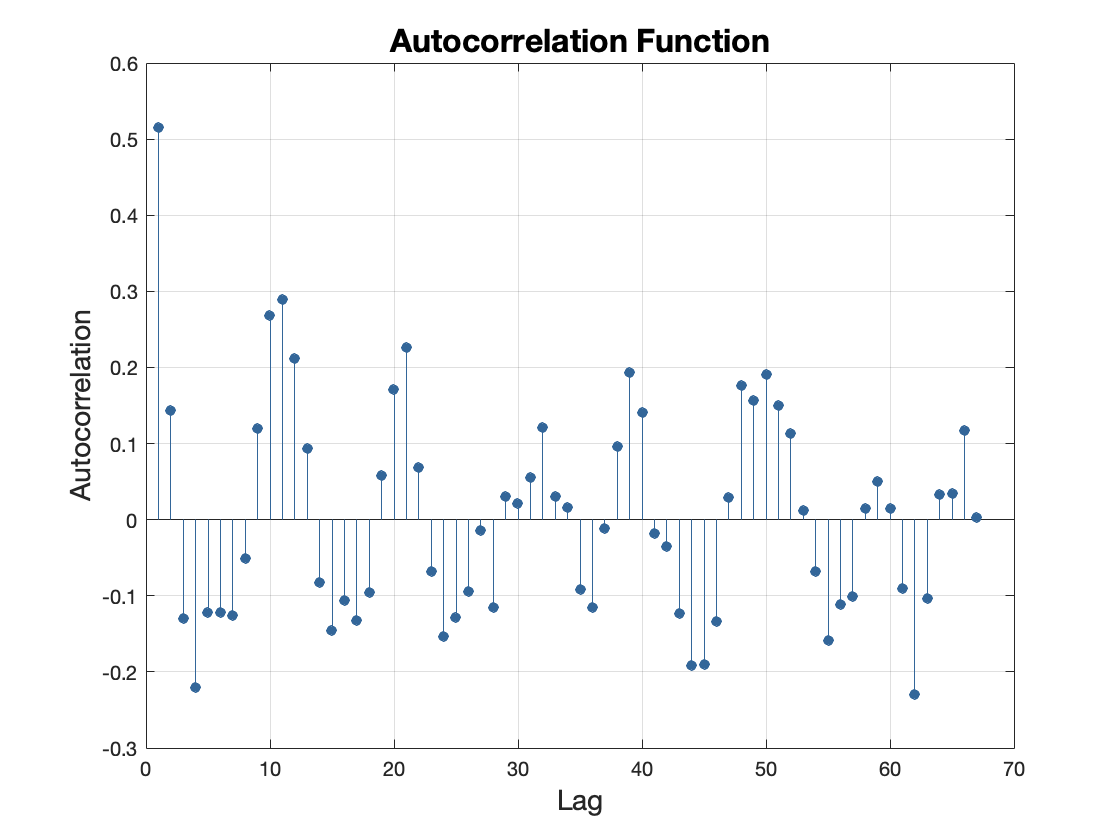
\includegraphics[width=\linewidth]{mainmatter/photos/momen_selfco_3.png}
        \caption{autocorrelation in match 3}
    \end{subfigure}
    \caption{Momentum autocorrelation}
    \label{fig:Correlation}
\end{figure}

The corrcoef of lag 1 in match one is 0.4546, match two 0.5149,match three 0.5342.
It can be seen that the autocorrelation of lag one is high, which means that the momentum at this moment
has a strong relationship with the momentum in the next round. And the autocorrelation decreases to random 
as the lag increases.

\subsubsection{correlation with runs of success}~{}

To give a quantitative evaluation of ``future scores'', we count points gain in future multiple rounds,
and derive the difference by minus that of the opponent. 
For example, if the player gains 3 points in the next 5 rounds, and the opponent gains 2 points,
the difference is 1.
The difference indicates how much better the player is performing than the opponent.

In intuition, the player with higher momentum should have a higher chance to win the next round.
And momentum at this moment should have less impact on the future rounds as time extends.
The correlation between momentum and future scores verifies our intuition.

We calculate points gain difference in future one to five rounds at each time of all matches.
Here we display five points gain difference and momentum difference in first three games.

\begin{figure}[H]
    \centering
    \begin{subfigure}[b]{0.34\textwidth}
        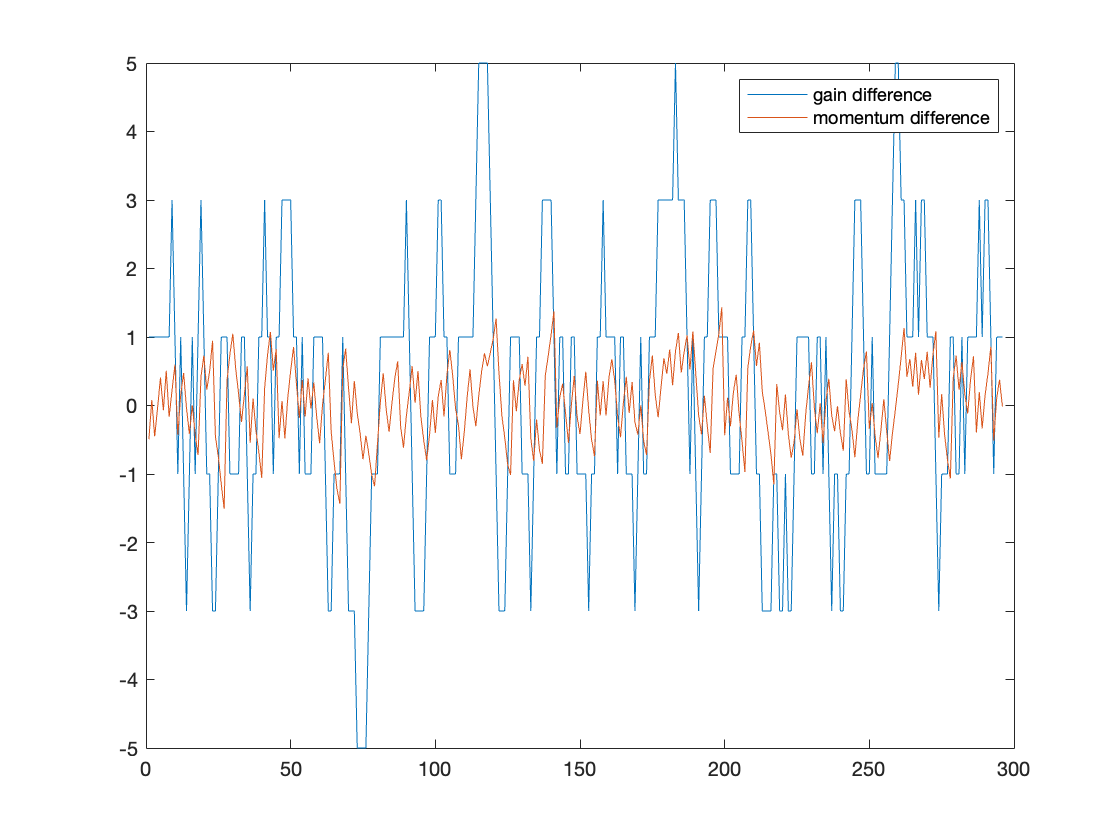
\includegraphics[width=\linewidth]{mainmatter/photos/diff_match1.png}
        \caption{2023-wimbledon-1301}
    \end{subfigure}\hspace{-0.02\textwidth}
    \begin{subfigure}[b]{0.34\textwidth}
        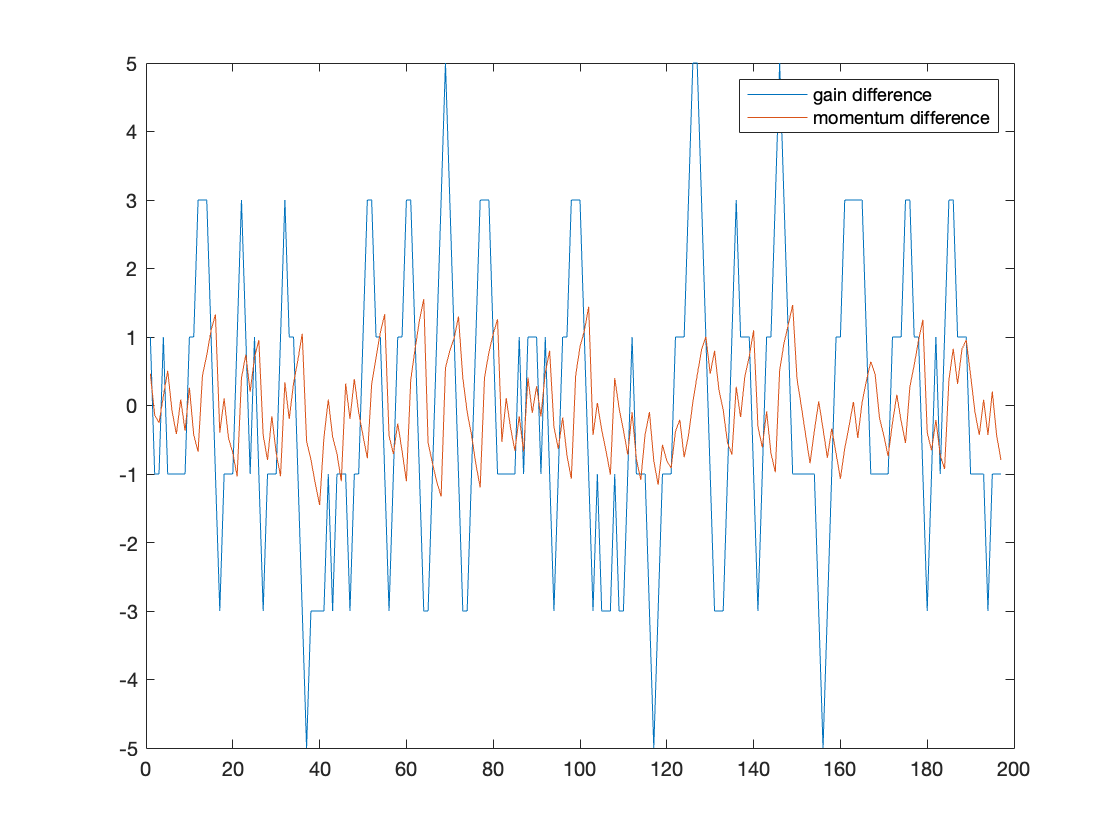
\includegraphics[width=\linewidth]{mainmatter/photos/diff_match2.png}
        \caption{2023-wimbledon-1302}
    \end{subfigure}\hspace{-0.02\textwidth}
    \begin{subfigure}[b]{0.34\textwidth}
        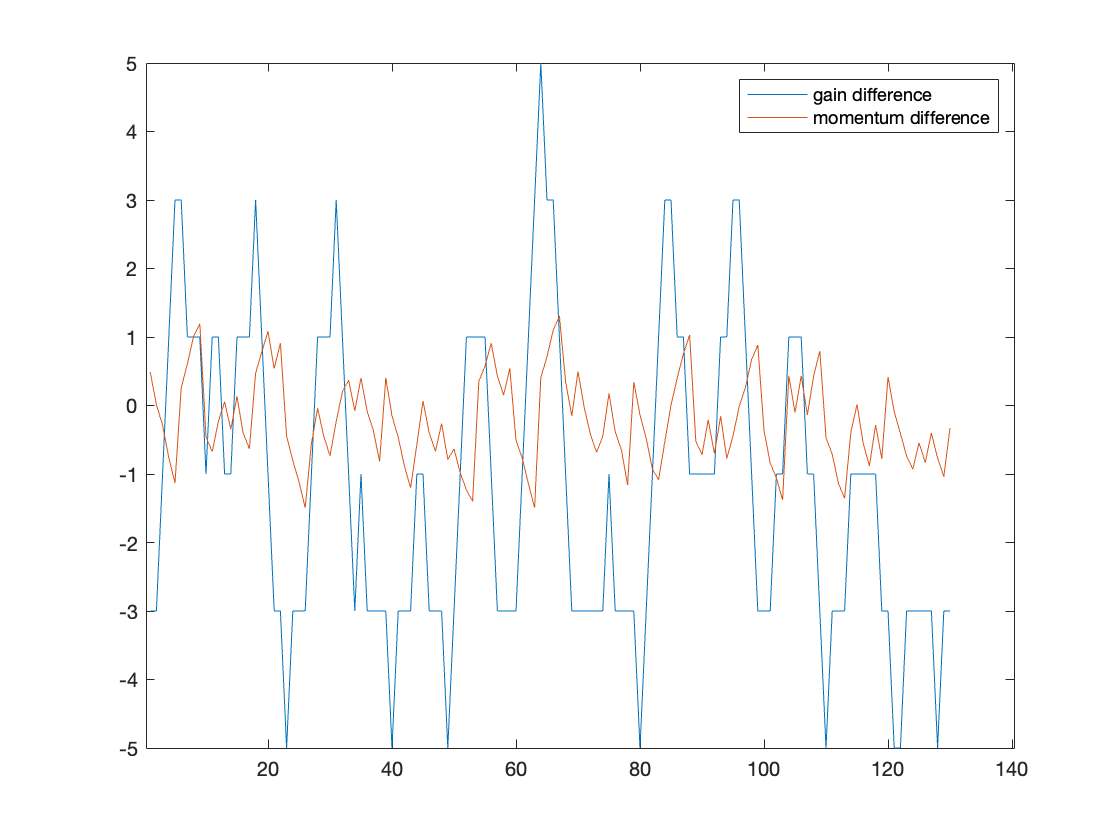
\includegraphics[width=\linewidth]{mainmatter/photos/diff_match3.png}
        \caption{2023-wimbledon-1303}
    \end{subfigure}
    \caption{Gain Difference and Momentum in First Three Games}
    \label{fig:Gain Difference and Momentum}
\end{figure}

And we derive the correlation between gain difference from one to five rounds 
and momentum difference of all matches. Here we display the three of them.

\begin{figure}[H]
    \centering
    \begin{subfigure}[b]{0.34\textwidth}
        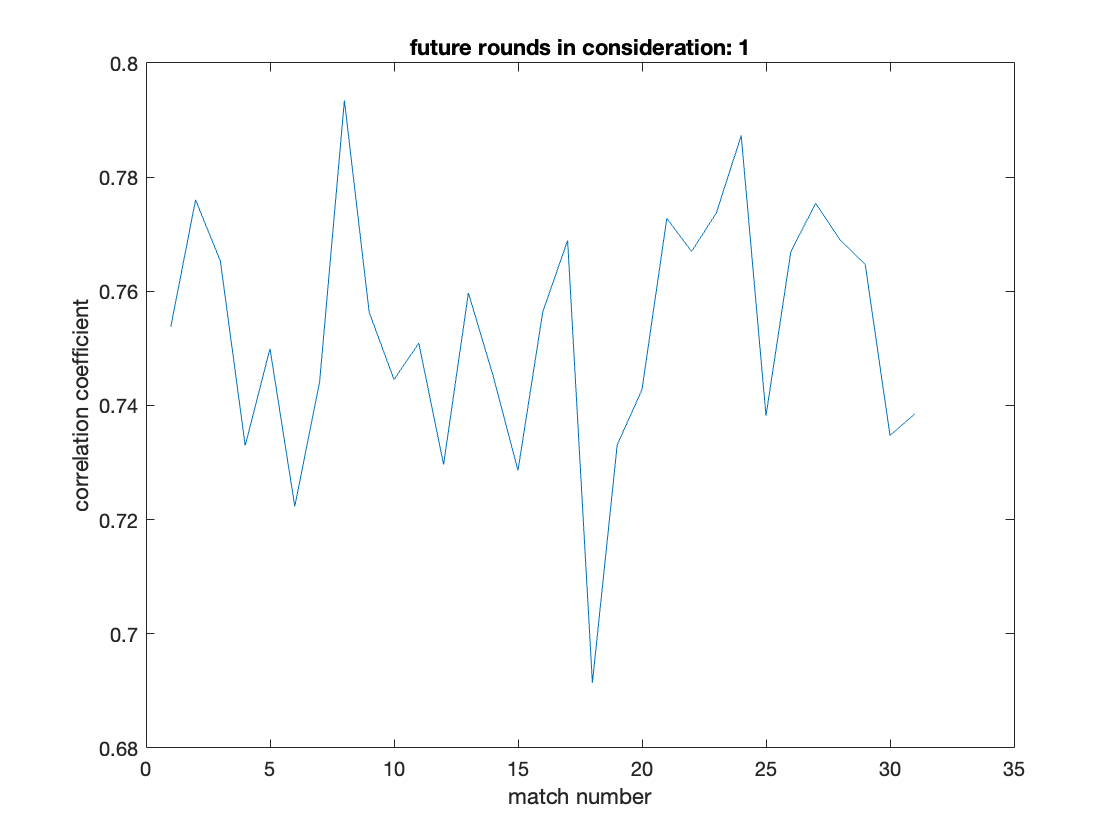
\includegraphics[width=\linewidth]{mainmatter/photos/momen_1points_cor.png}
        \caption{gain difference in 1 round}
    \end{subfigure}\hspace{-0.02\textwidth}
    \begin{subfigure}[b]{0.34\textwidth}
        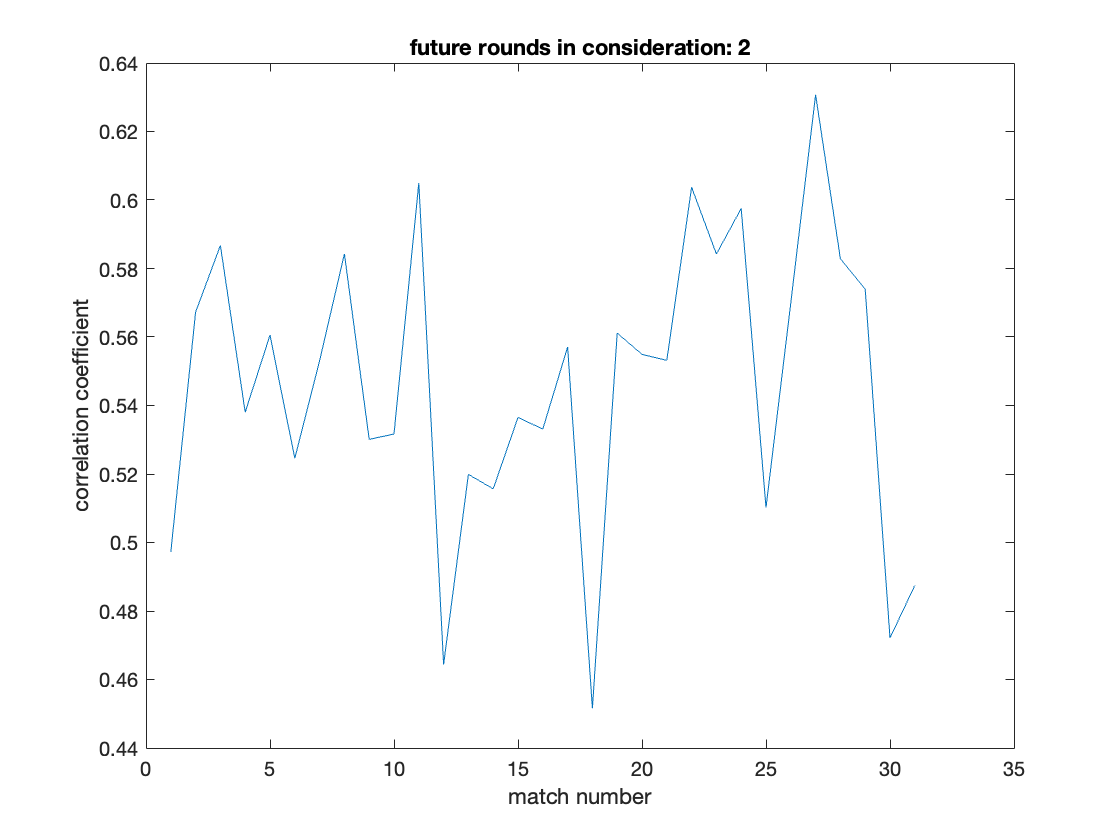
\includegraphics[width=\linewidth]{mainmatter/photos/momen_2points_cor.png}
        \caption{gain difference in 2 rounds}
    \end{subfigure}\hspace{-0.02\textwidth}
    \begin{subfigure}[b]{0.34\textwidth}
        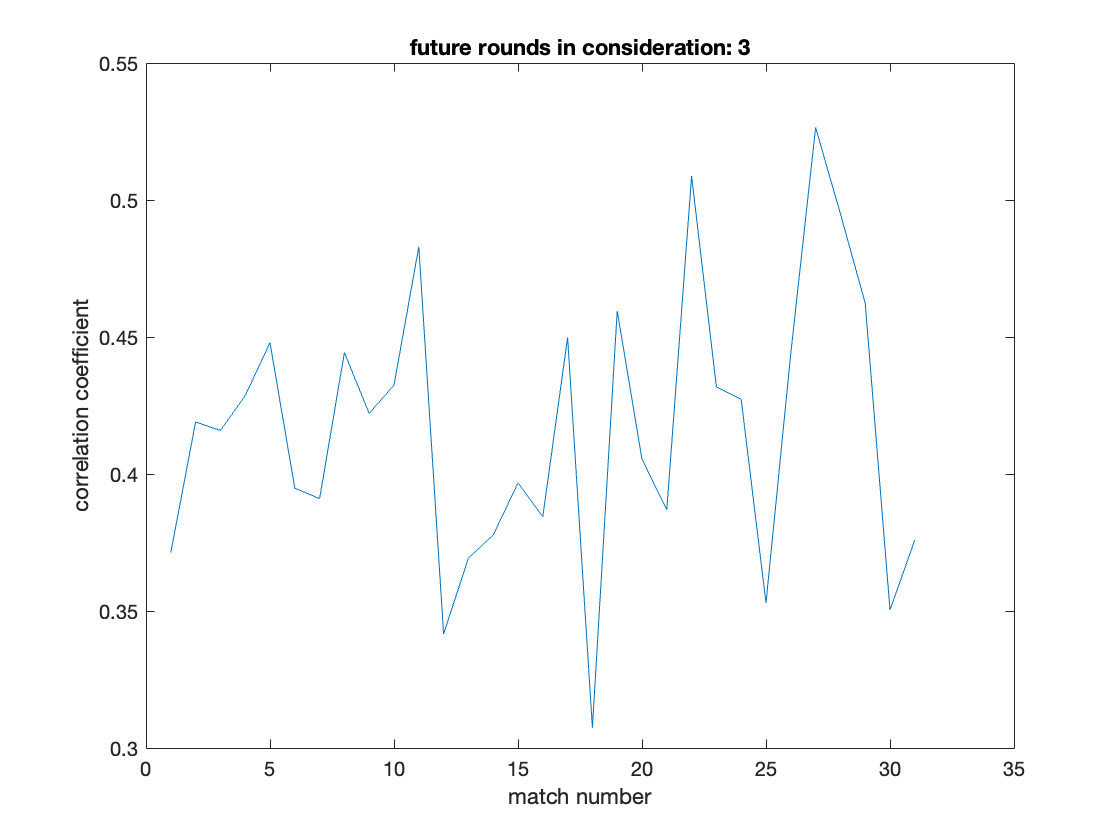
\includegraphics[width=\linewidth]{mainmatter/photos/momen_3points_cor.png}
        \caption{gain difference in 3 rounds}
    \end{subfigure}
    \caption{Correlation Between Gain Difference and Momentum Difference}
    \label{fig:Correlation}
\end{figure}

Here we display the max and min correlation in different rounds.
(hint. the max and min correlation means maximum and minimum of all matches.)

\begin{table}[!ht]
    \centering
    \begin{tabular}{|l|l|l|l|l|l|}
    \hline
        rounds & 1 & 2 & 3 & 4 & 5 \\ \hline
        max & 0.7934 & 0.6307 & 0.5264 & 0.4678 & 0.3910 \\ \hline
        min & 0.6914 & 0.4516 & 0.3074 & 0.1824 & 0.0627 \\ \hline
    \end{tabular}
    \caption{max and min Correlation of all matches in different rounds}
    \label{fig:maxmin Correlation}
\end{table}

As we can see from the table, the correlation between momentum and future scores is bigger
than 0.5 considering the next 1 round, it implies that momentum has a substantial impact on the next round.
And the correlation decreases as the rounds extend, which verifies our intuition, that
the momentum at this moment has less impact on the future rounds as time extends.

Now, we have finished problem 2.